\chapter{PILCO-style policy learning: full derivation and first results}
\textit{Archived October study. All simulations, searches, and checks described below predate this report.}\par

\section*{Chapter overview}
A Gaussian-process (GP) transition model and analytic Gaussian moment propagation are used to optimize a proportional-integral controller around an existing quadratic feedforward map. The benchmark is the previous 9250 rpm, sea-level, ISA-zero test with shaft-load pulses. Three historical controllers and the initial PI policy provide comparators. The selected gains are frozen before new nonlinear T-MATS simulations at 10\% and 5\% load amplitudes. This implementation is a PILCO-style, offline, single-model policy-improvement experiment: it uses numerical policy gradients, a fitted linear mean, a shared-kernel GP subset, and an expected quadratic cost. It is not an exact reproduction of the original PILCO training loop. All reported plant metrics come from saved nonlinear simulation traces, not GP rollout predictions.

\section{Experiment, provenance, and main result}
The chosen test is the most recent fixed-operating-point study in this workspace. The reference is 9250 rpm, altitude is 0 m, ISA deviation is 0 K, and Mach number is zero. Each simulation includes 60 s preparation and 90 s evaluation. The sample period is $h=0.015$ s. Turbine trim power is 15376.79195 hp; the 10\% disturbance is 1537.67919 hp. Relative to the evaluation start, load pulses occupy $[10.005,15)$, $[30,40.005)$, and $[60,75)$ s. Five-percent validation halves only the pulse magnitude.

The existing base PI, original Poly2, and retuned Poly2 traces are read from the previous study without alteration. The latter two include acceleration feedback (PID-like), so they are explicitly labelled as such. The new policy uses ordinary sensed-speed error and no derivative feedback.

The new nonlinear simulation has speed RMSE 1.1973 rpm, peak error 14.389 rpm, and fuel ringing 14.8252 lbm/s. Compared with retuned Poly2, tracking RMSE falls by 22.6\%, but ringing grows to 11.4 times its previous value. This is a tracking--actuation tradeoff, not an overall improvement.

\paragraph{Scope of the feedforward claim.} The quadratic coefficients are frozen from the prior inverse fit. PILCO learns the two PI gains, not the fifteen polynomial coefficients. At one fixed speed and ambient condition, feedforward is a constant and its offset is absorbed by bumpless integral initialization. Consequently this benchmark cannot identify a quadratic-map advantage over other constant feedforward values. The static map also slightly extrapolates: 9250 rpm is below its previous training-speed minimum of approximately 9264.23 rpm.

\section{Step 1: write the deployed control law}
Let $N_s$ denote sensed shaft speed, $r$ the governed reference, $T$ inlet temperature in kelvin, and $P$ inlet pressure in kPa. The old inverse model uses inputs $v=[N,\dot N,T,P]^\top$, standardized as $z_j=(v_j-\bar v_j)/s_j$. Its full quadratic is
\begin{equation}
 p_2(v)=c_0+\sum_{j=1}^4c_jz_j+\sum_{j=1}^4c_{jj}z_j^2+\sum_{i<j}c_{ij}z_iz_j.
\end{equation}
There are $1+4+4+6=15$ coefficients. Setting desired acceleration to zero defines static feedforward. The actual controller is
\begin{align}
 u_{\rm ff,k}&=p_2(r_k,0,T_k,P_k), &e_k&=r_k-N_{s,k},\\
 u_k^*&=u_{\rm ff,k}+K_pe_k+I_k, &u_k&=\operatorname{clip}(u_k^*,0.2,4),\\
 I_{k+1}&=I_k+hK_ie_k &&\text{when integration is permitted.}
\end{align}
Fuel is measured in lbm/s, $K_p$ in (lbm/s)/rpm and $K_i$ in (lbm/s)/(rpm s). Conditional integration permits an update if $(u^*<4\text{ or }e<0)$ and $(u^*>0.2\text{ or }e>0)$. Before 45 s the old controller supplies the command and the new integral tracks $I=u_{\rm old}-u_{\rm ff}-K_pe$. This gives a bumpless handover. Existing plant, sensor, request governor, load profile, solver and fuel limits are inherited by the new model copy.

\section{Step 2: construct the dynamics-learning state}
Use a dimensionless augmented state and a normalized load:
\begin{equation}
 x=\begin{bmatrix}(N-9250)/20\\(N-N_s)/5\\(I-I_0)/0.3\end{bmatrix},\quad
 d=\frac{P_{\rm load}}{1537.6791946},\quad I_0=u_0-u_{\rm ff}.
\end{equation}
The trim fuel $u_0=1.39529998$ lbm/s. The second state represents sensor lag; discarding it would make fast feedback dynamics less nearly Markov. At fixed reference,
\begin{equation}
 \tilde u=(u-u_0)/0.3=b^\top x,\qquad
 b^\top=\left[-\frac{20K_p}{0.3},\frac{5K_p}{0.3},1\right].
\end{equation}
The GP input is $z=[x_1,x_2,\tilde u,d]^\top=B x+a(d)$ and its output is the two physical-state increments $y=[\Delta x_1,\Delta x_2]^\top$. The integrator transition is known exactly, so learning it would waste data. With
\begin{equation}
 D=\begin{bmatrix}1&0&0\\0&1&0\\-20hK_i/0.3&5hK_i/0.3&1\end{bmatrix},\quad
 E=\begin{bmatrix}1&0\\0&1\\0&0\end{bmatrix},\qquad x^+=Dx+Ey,
\end{equation}
the feedback integral remains correlated with the turbine state during planning.

\section{Step 3: fit the probabilistic transition model}
Training uses transitions from the first two pulses of each historical controller: absolute windows $[69.9,78]$ and $[89.9,103]$ s. There are 4242 transitions. The third-pulse window $[119.9,138]$ s is held out for one-step dynamics checks. These trajectories share a deterministic plant and operating point; this is a temporal split, not independent hardware validation.

Fit a linear mean by least squares on training data only, $m(z)=a+Az$, and standardize each residual output with scale $s_j$. A deterministic farthest-point selection retains 40 representative GP inputs. For both standardized residual outputs, use the shared squared-exponential kernel
\begin{equation}
 k(z,z')=\sigma_f^2\exp\left[-\tfrac12(z-z')^\top\Lambda^{-1}(z-z')\right],\qquad
 \Lambda=\operatorname{diag}(\ell_1^2,\ldots,\ell_4^2).
\end{equation}
Let $K_n=K+\sigma_n^2\mathcal I+10^{-9}\mathcal I$ and let $R$ contain standardized residuals. Cholesky solves minimize the summed negative log marginal likelihood, up to constants:
\begin{equation}
 \mathcal L=\tfrac12\operatorname{tr}(R^\top K_n^{-1}R)+\frac{2}{2}\log|K_n|,\qquad \beta=K_n^{-1}R.
\end{equation}
The hyperparameter bounds in log units are $[-1,4]$ for length scales, $[-3,3]$ for signal standard deviation and $[-7,0]$ for noise standard deviation. Conditional on a deterministic input, residual outputs are independent and share covariance hyperparameters. Uncertain inputs induce output cross-covariance. The linear mean is treated as fixed: uncertainty in its estimated coefficients is not integrated out.

\section{Step 4: propagate a Gaussian through the policy}
Suppose $x\sim\mathcal N(\mu,\Sigma)$. For the unsaturated policy, the input moments are exact:
\begin{equation}
 m_z=B\mu+a(d),\qquad S_z=B\Sigma B^\top,\qquad C_{xz}=\Sigma B^\top.
\end{equation}
The load is a known deterministic scenario input during planning, not a measured feedforward input to the deployed policy. A full Gaussian may mathematically cross the fuel limits. Planning here uses the unsaturated affine policy; the nonlinear plant evaluation applies clipping and anti-windup. This is a local approximation, justified only to the extent that the evaluated commands remain inside the limits.

\section{Step 5: derive exact uncertain-input GP moments}
Write $m=m_z$, $S=S_z$, and let $z_i$ denote training inputs. Completing the square in the Gaussian integral of one kernel gives
\begin{align}
 q_i&=\int k(z,z_i)\mathcal N(z\mid m,S)\,dz\\
 &=\sigma_f^2\frac{|\Lambda|^{1/2}}{|S+\Lambda|^{1/2}}
 \exp\left[-\tfrac12(z_i-m)^\top(S+\Lambda)^{-1}(z_i-m)\right].
\end{align}
For two kernels, define $c_{ij}=(z_i+z_j)/2$ and $\delta_{ij}=z_i-z_j$. Their product separates into a distance factor and a Gaussian centered at $c_{ij}$. Therefore
\begin{align}
 Q_{ij}&=\E[k(z,z_i)k(z,z_j)]\\
 &=\sigma_f^4\exp[-\tfrac14\delta_{ij}^\top\Lambda^{-1}\delta_{ij}]
 \frac{|\Lambda/2|^{1/2}}{|S+\Lambda/2|^{1/2}}\nonumber\\
 &\hspace{7mm}\cdot\exp[-\tfrac12(c_{ij}-m)^\top(S+\Lambda/2)^{-1}(c_{ij}-m)].
\end{align}
Let $g$ be the standardized residual GP output. The law of total expectation and total covariance now give
\begin{align}
 \bar g&=\beta^\top q,\\
 V_g&=\beta^\top Q\beta-\bar g\bar g^\top+
 \mathcal I\left[\sigma_f^2-\operatorname{tr}(K_n^{-1}Q)+\sigma_n^2\right].
\end{align}
The last term includes observation/model-residual noise in each predicted transition. Propagating this as temporally independent noise does not represent a single fixed GP function sample across the entire horizon. This standard moment-propagation approximation can accumulate model uncertainty differently from trajectory sampling.

The Gaussian kernel identity also yields
\begin{equation}
 G=(S+\Lambda)^{-1}\sum_i(z_i-m)q_i\beta_i^\top H,
 \qquad H=\operatorname{diag}(s_1,s_2).
\end{equation}
Then $\Cov(z,Hg)=SG$. Restoring the linear mean and residual scales,
\begin{align}
 \bar y&=a+Am+H\bar g,\\
 V_y&=ASA^\top+HV_gH+ASG+G^\top SA^\top,\\
 C_{xy}&=C_{xz}(A^\top+G).
\end{align}
The cross terms matter: dropping $C_{xy}$ loses the dependence between current state and predicted state increment. All inverses above involve a positive-definite kernel length-scale matrix added to $S$, so a singular $S$ from deterministic scenario inputs is allowed.

\section{Step 6: close the moment recursion}
Substitution into $x^+=Dx+Ey$ gives
\begin{align}
 \mu^+&=D\mu+E\bar y,\\
 \Sigma^+&=D\Sigma D^\top+EV_yE^\top+DC_{xy}E^\top+EC_{xy}^\top D^\top.
\end{align}
Each transition is then approximated by a Gaussian with these moments. This preserves first and second moments of the one-step mapping under the Gaussian input assumption; it does not preserve multimodality of the true multistep distribution. Initial planning moments are $\mu_0=0$ and $\Sigma_0=\operatorname{diag}(10^{-6},10^{-6},10^{-8})$.

\section{Step 7: derive and optimize the expected cost}
For a 5 s planning horizon at the same 15 ms sample period, a unit load pulse is applied for $1\le t<2.5$ s. The objective is
\begin{align}
 J(\theta)&=h\sum_k\E[x_{1,k}^2+0.01\tilde u_k^2]\\
 &=h\sum_k\left[\mu_{1,k}^2+\Sigma_{11,k}+0.01\{(b^\top\mu_k)^2+b^\top\Sigma_kb\}\right].
\end{align}
Use $\theta=[\log K_p,\log K_i]^\top$, so gains remain positive. Bounds are $0.005\le K_p\le0.07$ and $0.01\le K_i\le0.25$. The initial policy is $(0.025,0.05)$. L-BFGS-B repeatedly evaluates the complete Gaussian rollout and estimates parameter gradients numerically. The conceptual chain rule is
\begin{equation}
 \frac{dJ}{d\theta}=\sum_k\left(\frac{\partial J}{\partial\mu_k}\frac{d\mu_k}{d\theta}+\frac{\partial J}{\partial\Sigma_k}:\frac{d\Sigma_k}{d\theta}+\frac{\partial J}{\partial\theta}\right).
\end{equation}
For implementation, this derivative is approximated by finite differences of the full objective rather than hand-coded analytic sensitivities. The learned result is
\begin{equation}
 \boxed{K_p=0.06460568,\qquad K_i=0.17102610,\qquad K_d=0.}
\end{equation}
Expected cost changes from 0.464463 to 0.141314. This cost is dimensionless and is not the reported full-test speed RMSE or fuel-ringing metric. Gains are frozen immediately after optimization; no 5\% validation result is used in selection.
\begin{figure}[H]\centering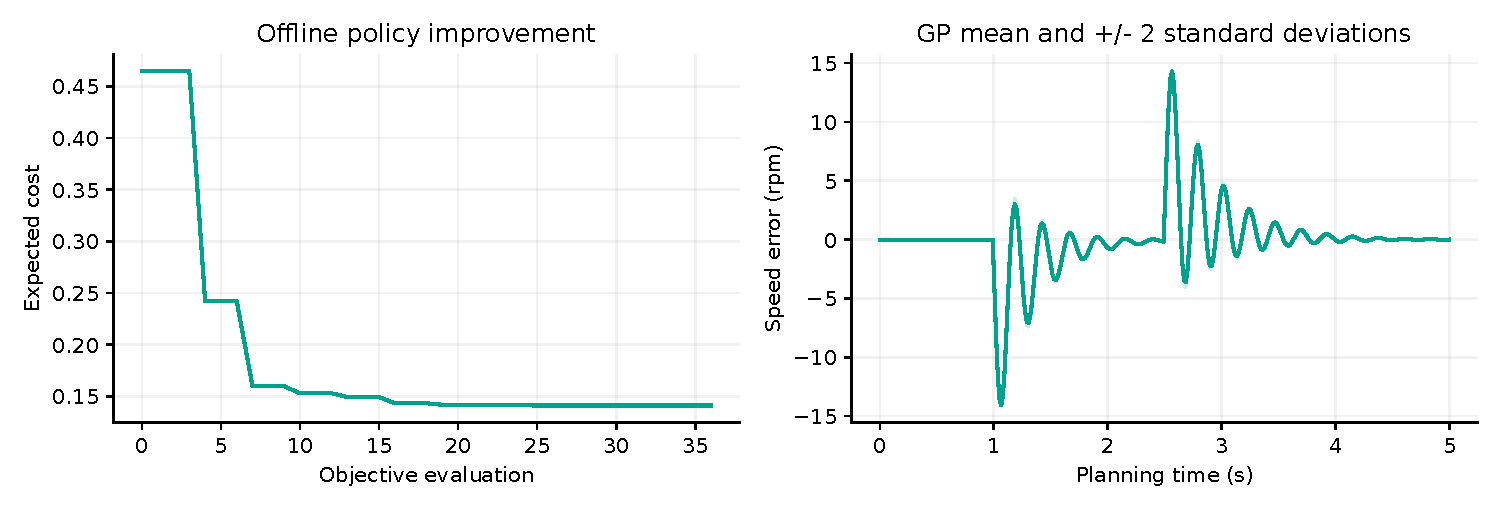
\includegraphics[width=\linewidth,height=.68\textheight,keepaspectratio]{late0_learning.pdf}\caption{Policy-search objective and GP planning response. The shaded interval is model uncertainty, not a certified plant confidence band.}\end{figure}

\section{Step 8: nonlinear plant comparison and independent checks}
All three new simulations use the copied T-MATS plant: selected policy at 10\%, selected policy at 5\%, and initial quadratic-feedforward PI at 10\%. Historical traces supply the three earlier comparators. The initial-policy ablation helps distinguish gain learning from merely adding a constant feedforward value. File hashes and replay checks are saved with the study.

\begin{table}[H]\centering\small\begin{tabular}{lrrrr}\toprule Controller & RMSE & Peak & Ringing & Settling\\ & rpm & rpm & lbm/s & s\\\midrule
Base PI & 2.4209 & 21.406 & 2.0702 & 2.475 \\
Original Poly2 + PID & 1.6658 & 14.113 & 1.6968 & 1.365 \\
Retuned Poly2 + PID & 1.5461 & 15.825 & 1.2990 & 0.930 \\
PILCO FF+PI & 1.1973 & 14.389 & 14.8252 & 1.920 \\\bottomrule\end{tabular}\caption{10\% load-amplitude comparison.}\end{table}
\begin{table}[H]\centering\small\begin{tabular}{lrrrr}\toprule Controller & RMSE & Peak & Ringing & Settling\\ & rpm & rpm & lbm/s & s\\\midrule
Base PI & 1.1692 & 10.392 & 1.0583 & 2.115 \\
Original Poly2 + PID & 0.8018 & 6.969 & 0.9005 & 1.260 \\
Retuned Poly2 + PID & 0.7439 & 7.806 & 0.6544 & 0.870 \\
PILCO FF+PI & 0.5930 & 7.008 & 7.9471 & 1.695 \\\bottomrule\end{tabular}\caption{5\% load-amplitude comparison.}\end{table}

RMSE uses every sample in $[60,150]$ s. Peak error is maximum absolute speed error in that interval. IAE uses the same rectangular sample sum as the prior report. Fuel ringing sums, over six two-second event windows, total variation minus absolute net fuel change:
\begin{equation}
 R=\sum_{j=1}^{6}\left[\sum_{k\in W_j}|u_{k+1}-u_k|-|u_{\mathrm{last}(j)}-u_{\mathrm{first}(j)}|\right].
\end{equation}
This is a reversal metric in lbm/s, not fuel consumed. Settling requires persistent entry into $\pm0.1$ rpm until the next event. Numerical acceptance checks full duration, finite signals, positive fuel, positive surge margin, flow residual at most $10^{-9}$, fewer than 200 solver iterations, and pre-test speed within 0.1 rpm.

The analytic GP covariance agrees with a 50,000-input Monte Carlo integration to 0.31\% relative Frobenius error; input/output cross-covariance error is 1.57\%. Held-out one-step speed-increment RMSE ranges from 0.000432 to 0.000709 rpm. Independent command and integral replay errors are below $10^{-8}$. All evaluated new traces pass the existing numerical acceptance checks. The selected 10\% run has minimum surge margin 14.800\% and fuel saturation fraction 0.000\%.
\begin{figure}[H]\centering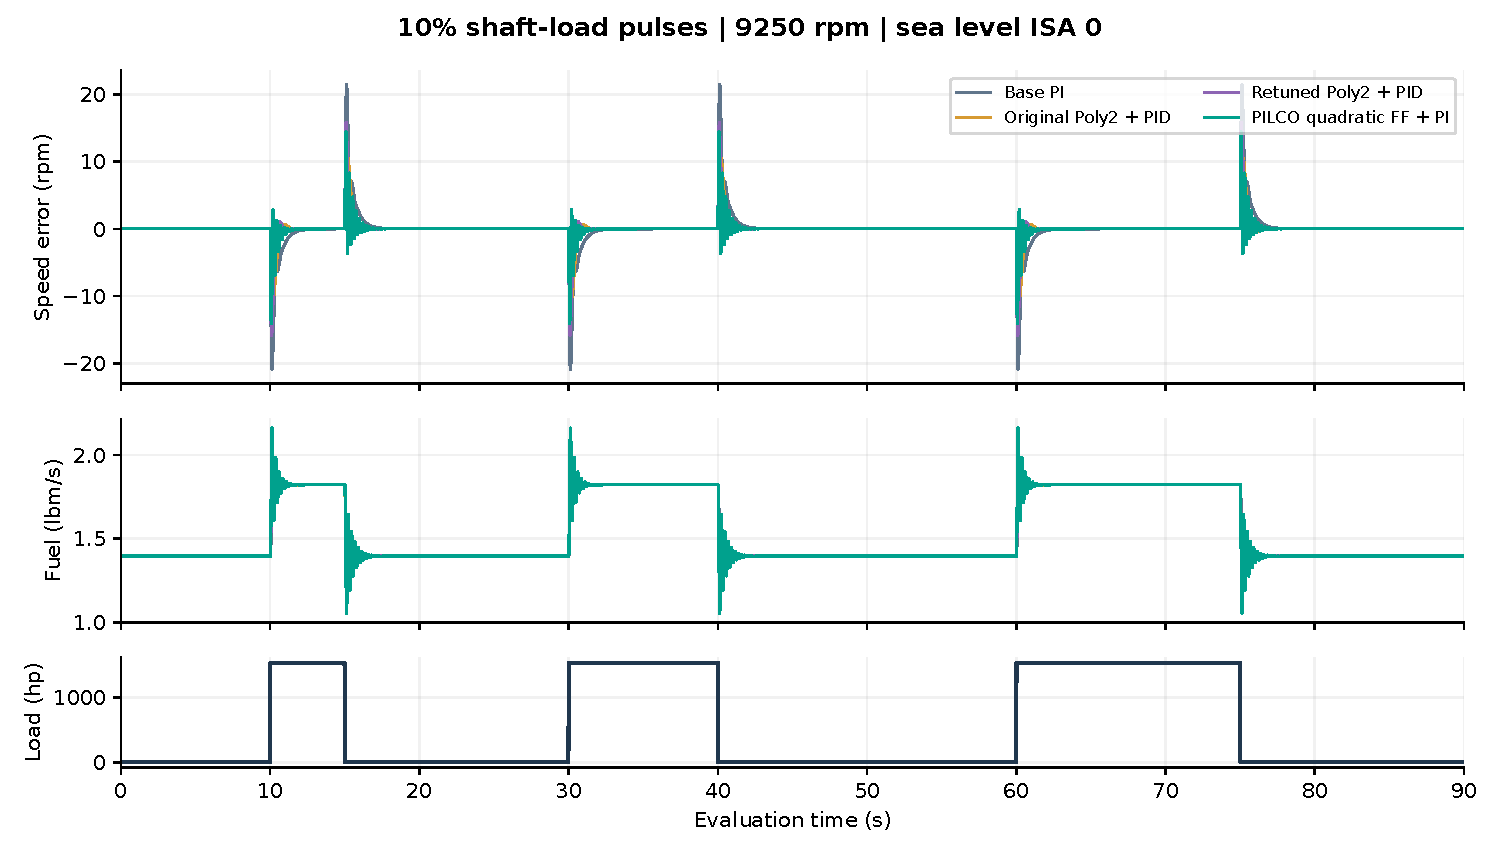
\includegraphics[width=\linewidth,height=.68\textheight,keepaspectratio]{late0_comparison_10pct.pdf}\caption{Full nonlinear 10\% benchmark. Historical methods and new controller use matching time, request and disturbance profiles.}\end{figure}
\begin{figure}[H]\centering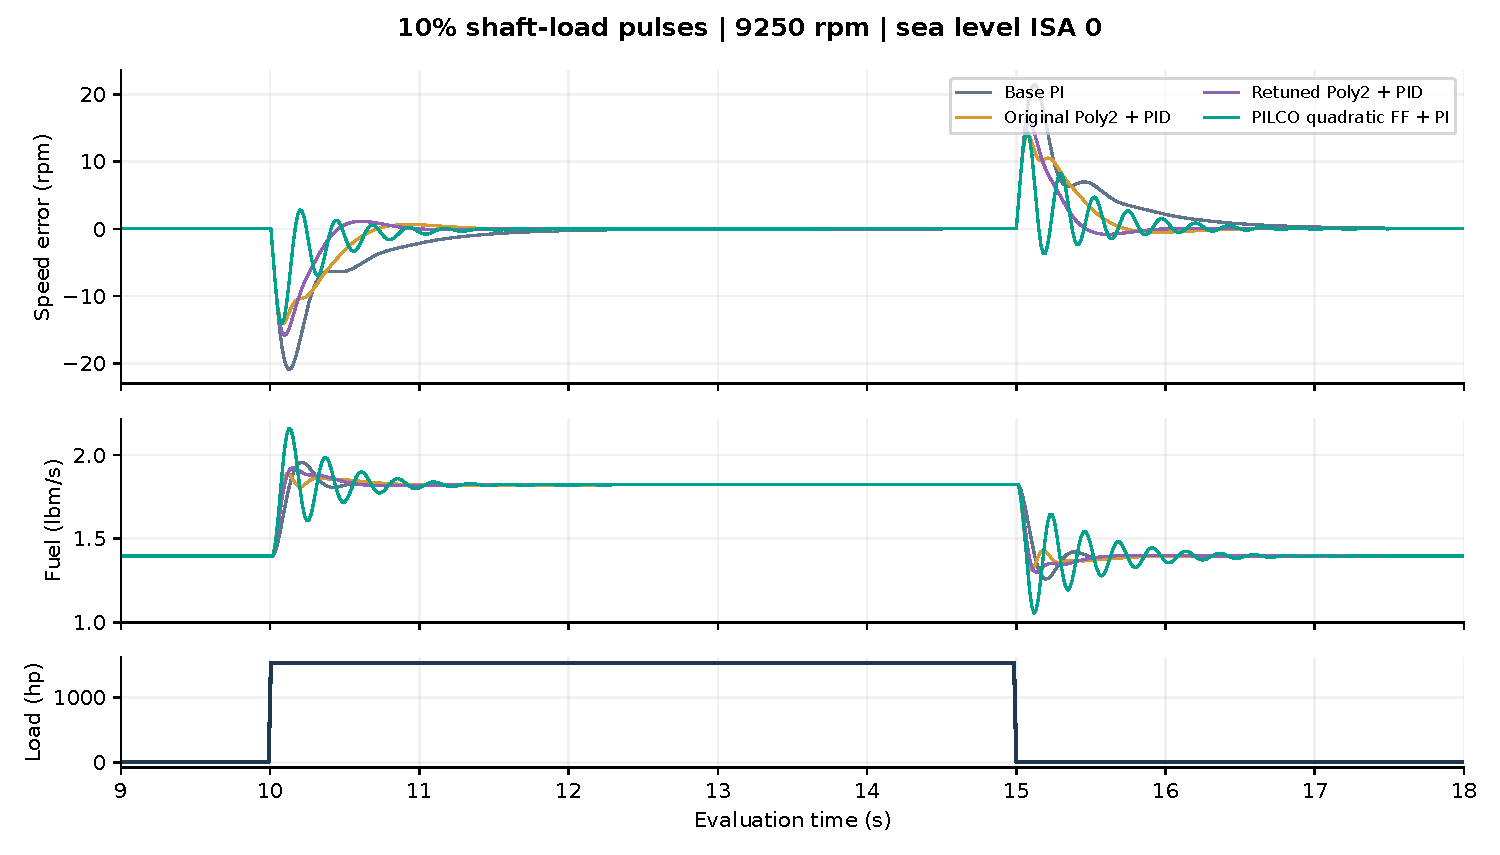
\includegraphics[width=\linewidth,height=.68\textheight,keepaspectratio]{late0_zoom_10pct.pdf}\caption{First pulse, emphasizing overshoot and command reversals. The new method is judged on these plant traces.}\end{figure}
\begin{figure}[H]\centering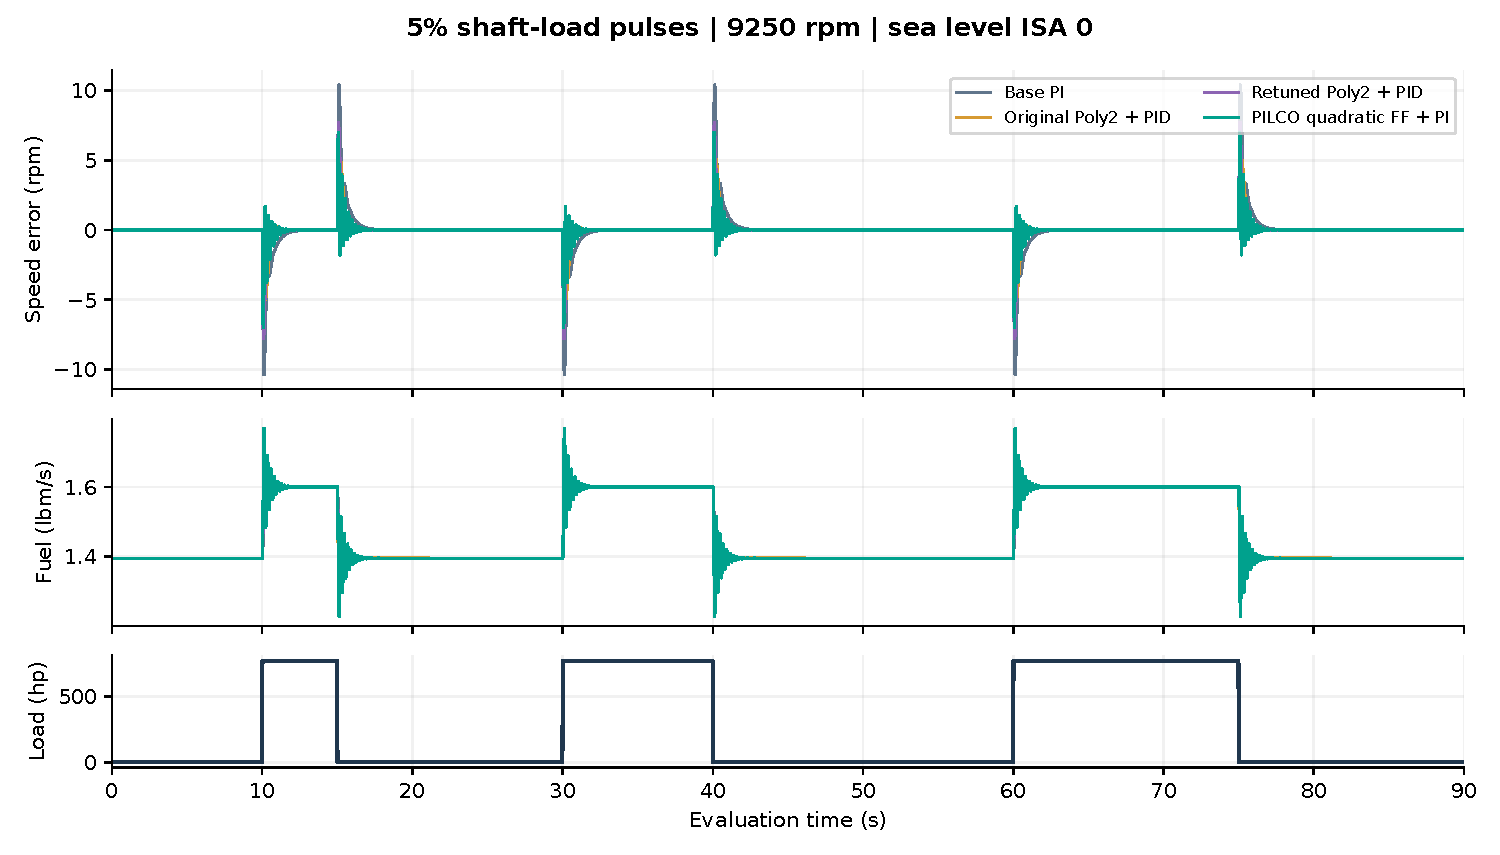
\includegraphics[width=\linewidth,height=.68\textheight,keepaspectratio]{late0_comparison_5pct.pdf}\caption{Frozen-policy 5\% amplitude validation at the same operating point.}\end{figure}

\section{Interpretation and limitations}
Relative to Base PI, RMSE changes by -50.5\% and ringing by +616.1\%. Relative to Retuned Poly2 + PID, RMSE changes by -22.6\% and ringing by +1041.2\%. The initial feedforward PI has RMSE 2.4406 rpm and ringing 2.0296 lbm/s. These quantities describe different tradeoffs; minimizing expected tracking cost does not directly minimize fuel reversals.

The original PILCO method uses GP dynamics, uncertainty-aware long-horizon prediction and policy search with analytic gradients~\cite{pilco}. This study retains GP moment matching but changes the policy family, cost, mean function, training source and gradient implementation. It performs one offline improvement round using existing experiments; it does not claim learning from scratch or a repeated collect--refit--improve loop. Forty representative GP points are a subset approximation, and a low held-out one-step error does not establish calibrated long-horizon uncertainty. The moment check validates the algebra against integration, not the physical accuracy of the GP.

The local state omits thermodynamic internal states; the linear mean and GP can absorb only their effects visible in the training trajectories. The deployment sensor dynamics are inherited from the plant, while learning identifies their observed effect. No guarantee of global stability, robustness at other speeds or ambient conditions, or hardware safety follows from these simulations. A multi-speed test with a frozen validation protocol would be required to assess the quadratic feedforward surface itself. The video is an animation of recorded signals; rotor speed is visually scaled and is not a blade-resolved turbine simulation.

\section{Reproduction and delivered files}
The source scripts are \path{pilco_tmats.py} (GP and policy learning), \path{tmats_pilco_pi_sfun.m} (deployed controller), \path{tmats_pilco_setup.m}, \path{run_tmats_pilco.m} (plant runs), and \path{build_pilco_deliverables.py} (verification, figures, paper and video). The ready-to-open model is \path{GasTurbine_PILCO_Quadratic_PI.mdl}. It requires the existing adjacent T-MATS library and the frozen fit files in this workspace.

Run Python learning first, then execute \path{run_tmats_pilco} in MATLAB R2018b or a compatible release. Finally run the artifact builder. The results directory contains policy JSON, GP parameters, search history, prediction moments, MAT/CSV plant traces, comparison metrics, replay verification and a hash manifest. The paper source and figures are included alongside the PDF. Re-running overwrites only this study's outputs; preserve them first if a second independent run is desired.

